\chapter{Background}
\label{ch:background}

This chapter presents the necessary background information for this thesis. First, we define some basic terminology that we use throughout this document. Next, we research prior work in the field of \acrshort{vr} that interfaces \acrshort{vtk} and Unity or develops \acrshort{ide}s for visualizations within a \acrshort{vr} environment. We also examine the software and solutions produced by these previous studies and extract which factors contribute to potential maintainability issues and which on the contrary make them more maintainable. 

\section{Terminology}

We define a set of terms that we use throughout this thesis. We use the \textit{Glossary of virtual reality terminology} \cite{manetta1995glossary} as a main source for our terminology.

\begin{itemize}[leftmargin=1.5truecm]
    \setlength{\itemindent}{-1truecm}
    \item[] \textbf{\acrfull{vr}} A computer system used to create an artificial world which is immersive and interactive for the user.
    \item[] \textbf{Immersion} The feeling of the user of being part of a virtual environment.
    \item[] \textbf{Virtual Environment} Realistic simulations of interactive scenes.
    \item[] \textbf{Interactivity} The ability of the user to navigate and manipulate (objects in) the environment.
    \item[] \textbf{Visualization Toolkit} Library containing functionality aimed at creating and manipulating data visualizations.
    \item[] \textbf{Game Engine} A software that enables the creation of virtual environments.
\end{itemize}

\section{The Visualization Toolkit}

As the necessity to produce ever more complex visualizations grows, both in commercial and scientific settings, a number of visualization toolkits have been developed to support the development of these visualizations. These libraries tend to specialize on some form of visualization; for example, \acrfull{vtk} focuses on scientific visualization \cite{kruis_creating_2017}.

These toolkits come in a variety of flavours, languages and/or wrappings and it is thus out of the scope of this thesis to analyse and develop upon all of them. We discuss research done on all three to create \acrshort{ide}s for or within \acrshort{vr} environments, but we ultimately choose to use for a proof of concept.

\acrfull{vtk} is a library oriented towards \blockquote{\textit{manipulating and displaying scientific data}}\footnote{\url{https://vtk.org/}}. It creates visualizations by means of filter pipelines, a technique proposed by Haber and McNabb \cite{haber1990visualization}. These filters manipulate input data through some set of transformations and return the composed data which can then be visualized. 

\acrshort{vtk} has three different stages of the pipeline which combined return a visualization rendering. The first stage is the generation or the import of a data source and transforming the raw data in some more readable raw data if needed, like structuring it in a model. Subsequently, the raw data is then transformed through filters that compose the data in order for it to be visualized, creating the actual visualization. Finally, the visualization is rendered through the application of mappers that transform the computational representation into a graphical representation. An example of a Quadric 3D function is shown in Figure~\ref{fig:quadric-render-pipeline}, based on an example proposed in the \acrshort{vtk} example repository\footnote{Available at \url{https://kitware.github.io/vtk-examples/site/Cxx/VisualizationAlgorithms/ContourQuadric/}.}, the exact code is presented in Appendix~\ref{apx:quadric-vtk}.

\begin{figure}[t]
    \centering
    \begin{subfigure}{\textwidth}
        \centering
        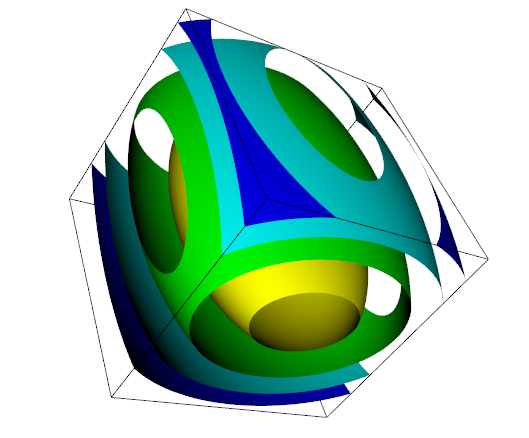
\includegraphics[width=0.7\textwidth]{pictures/Quadric-Rendering.PNG}
        \caption{}
    \end{subfigure}
    \begin{subfigure}{\textwidth}
        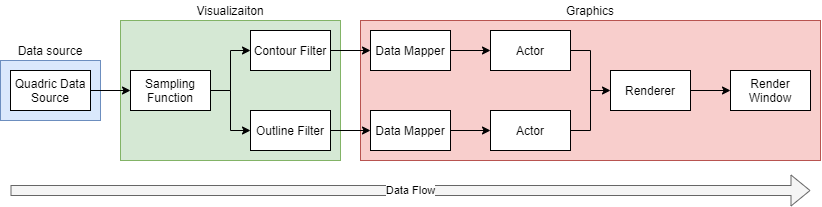
\includegraphics[width=\textwidth]{pictures/Pipeline-VTK-Quadric.png}
        \caption{}
    \end{subfigure}
    \caption{VTK visualization (a) and pipeline (b) of a sampled Quadric function.}
    \label{fig:quadric-render-pipeline}
\end{figure}

Upon \acrshort{vtk}, a number of wrappers have been produced, allowing the library to be used not only in C++, but also in Java, Python, Tcl and the .NET Framework\footnote{\url{https://vtk.org/Wiki/VTK/Wrappers}}. These wrappers allow the usage of the \textit{wrappable} code of the library from one of the aforementioned languages. This process is to be manually done at build time of the library or using one of the wrapping tools accessible from the documentation of \acrshort{vtk}.

\section{Unity Game Engine}

Game Engines can be defined as "\textit{software frameworks for game development}" \cite{politowski2021game}. These frameworks though are not all equal, and as such we focus on those defined as \textit{\acrfull{gpge}s}, which we define as \textit{frameworks for the creation of virtual environments}, which is a fundamental component of games. This also means that these softwares are not restricted to game development purposes, but are used for a variety of projects that entail the simulation of virtual worlds. These frameworks perfectly fit our requirement of creating an immersive and interactive environment for our \acrshort{vr} IDE.

A number of \acrshort{gpge}s exist, such as Unity Engine \cite{haas2014history} and Unreal Engine \cite{unrealengine}. We use Unity as the engine on which we base our solution. This is ideal for our research as previous research already exists discussing the integration of \acrshort{vtk} and this engine \cite{wheeler_virtual_2018}. Furthermore, it is a very well established, used and supported engine.

We chose to use Unity due to the number of advantages that come with the engine. First and foremost, Unity has already a decent \acrshort{vr} integration with the OpenVR\footnote{\url{https://github.com/ValveSoftware/unity-xr-plugin}} and OpenXR\footnote{\url{https://docs.unity3d.com/Packages/com.unity.xr.openxr@0.1/manual/index.html}} plugins. The \acrshort{vr} community is already quite established and, in general, the development community is very active and offers valuable support. 

The documentation for the engine is comprehensive and freely available with a number of examples that facilitate development, and its API supports the implementation of custom native C++ code through easy drag-n-drop of the shared libraries in the editor and an intuitive interface to import its functionalities in C\#. Finally, thanks to OpenGL 2 context sharing, it is possible to render through external code, such as \acrshort{vtk}, which suites our need to visualize objects created in native C++ libraries.

\section{HTC Vive Headmounted Display}

Our objective is to have a generic environment that can be used with any HMD. For our development, however, we focus on the HTC Vive series as these are the HMDs we have access for development and testing. These VR headsets have a 90 Hz refresh rate on the entire line and can be used with controllers, allowing for interactive usage. In particular we focus on the HTC Vive, that we use for both development and testing. This headset is shown in Figure~\ref{fig:htc-vive}

\begin{figure}[t]
    \centering
    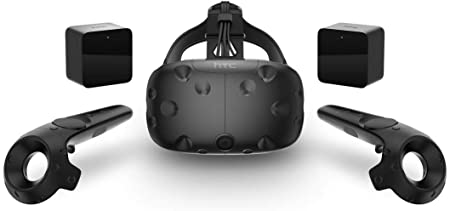
\includegraphics[width=.7\textwidth]{pictures/htc_vive.jpg}
    \caption{HTC Vive HMD with cameras and controllers.}
    \label{fig:htc-vive}
\end{figure}

\section{Related Work}
\label{sec:related-work}

A number of projects already attempted interfacing visualization libraries with frameworks, be it \acrshort{gpge}s or IDEs, while others attempted the creation of visualization editors, albeit for different purposes and/or constraints. In this section we discuss these previous attempts and how they contribute to laying the ground for our development.

\paragraph{OculusVTK Visual editor}

, developed in 2016, is a similar attempt to create a visual editor for OculusVTK carried out in Python \cite{dreuning_visual_2016}. The solution allows the user to create simple pipelines and manipulate them within a visual environment and see the result of the operations. The authors carry out a number of experiments with pipelines, varying from simple arrows to stream tracers and a DICOM image rendering, where results showed a consistent 58-60 FPS were achieved.

While the objectives of the authors are quite similar to ours, they do not focus on the same constraints we set for our project, i.e. performance and the designing of a distributable and parallelizable architecture. Furthermore, their solution focuses on Oculus, whereas our solution aims at being headset-agnostic.

The power of the solution proposed lays in its usage of Python's capability of introspecting on its modules and harvesting data in order to achieve a more general approach to interfacing with \acrshort{vtk}. We base our solution partly on this software, as we discuss in Section~\ref{sec:design-introspection}.

% Cannot find any reference of OculusVTK outside of one SURFsara webpage and Dreuning's and Perlee's theses.
On the other hand, this solution is limited to the usage of the OculusVTK C++ boilerplate for OculusVR. The code is maintained by SURFsara and offers an extension of the OculusVR SDK for Oculus HMDs. Compared to the support of Unity, this limits the generality of the solution, which we aim at extending.

Also due to the usage of OculusVTK, the solution proposes a complex building system prone to errors and issues related to building platforms, versions and library installations. Our objective is to streamline the building of our solution, if any is needed, and make our solution version-agnostic towards its dependencies. 

Furthermore, the Python scripts are limited to only working through introspection on \verb|vtkAlgorithm| subclasses, which limits the user to using such powerful tool on a subset of all available features of VTK. We aim at a general solution, thus either extending the approach up to any \verb|vtkObjectBase| subclass or to allow access to other features through the offered API.

\paragraph{VtkToUnity} is the closest attempt to our project was presented in 2018 by Wheeler et al. \\
\cite{wheeler_virtual_2018}. who developed a Native Unity plugin that allowed the user to exploit \acrshort{vtk}'s features in the engine's scripts\footnote{\url{https://gitlab.com/3dheart_public/vtktounity}}. The plugin's aim is to introduce volume rendering through \acrshort{vtk} and uses the OpenGL context sharing technology to enable the visualization library to directly render within the Unity scene. The plugin's approach is to add a rendering callback function after the transparency rendering stage, as optimal for volume rendering. The produced architecture is summarized in Figure~\ref{fig:wheeler-architecture} 

\begin{figure}[t]
    \centering
    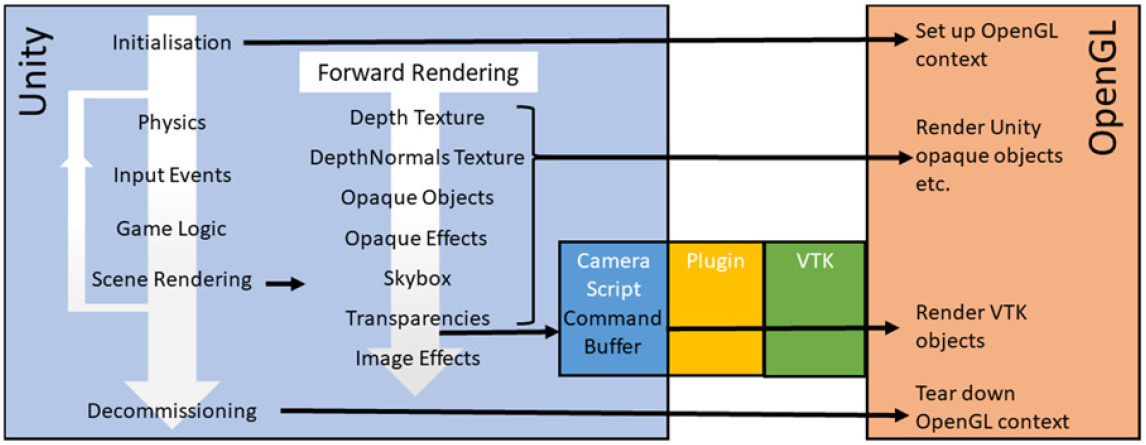
\includegraphics[width=\textwidth]{pictures/wheeler_arch.PNG}
    \caption{Wheeler et al.'s rendering architecture.}
    \label{fig:wheeler-architecture}
\end{figure}

The authors carry out experiments to evaluate the performances of the solution. Their objective frame rate is of 90 FPS using a HTC Vive \acrfull{hmd}, which aligns with Unity's own guidelines \cite{unity_vr_2020} as well as the 90Hz refresh rate of the \acrshort{hmd} \cite{BuyVIVEH54}. With simpler renderings the solution is of its own able to achieve the desired frame rate, but with more complex scenes it does not. To overcome this, the authors propose the usage of setting the desired frame rate using \acrshort{vtk}'s own \verb|vtkExternalRenderingOpenGLRenderWindow::SetDesiredUpdateRate| to solve this.

This solution presents some limitations, as the C++ native code locks the shared API at every call, and as such limits the ability to leverage parallelization of the software, which could potentially aid the rendering quality while the objective frame rate is set. Furthermore, the plugin focuses on volume rendering in particular, while our solution aims at a more general solution.

An issue with the maintainability of the VtkToUnity plugin is its hardcoding of features and reliance on patches to \acrshort{vtk}'s code to make it work correctly. For a specific application this is not a problem, but as our objective is to offer a generic solution to access VTK from Unity, this is not viable, as it introduces couplings to versions and particular algorithms and pipelines, and the potential for bugs and clones.

Our solution aims at creating a bridge that would allow the user to create pipelines in Unity without having hardcoded features limiting the user capabilities.

\paragraph{ActiViz}\footnote{\url{https://www.kitware.eu/activiz/}} is a \acrshort{vtk} wrapper for .NET, developed by Kitware, the company that is also mantaining \acrshort{vtk}. This wrapper is ready to be used with Unity, and exposes the same functionality of the library as other wrappers. This allows already for a good integration of the library and Unity.

The downside of this solution is its performance: as the wrapper requires CPU to GPU copies, with complex visualizations the performances drop significantly. This has already been discussed by Wheeler et al. \cite{wheeler_virtual_2018} and is one of the reasons that lead them to develop their own solution. On the other side, this is an official wrapper maintained by Kitware, the same creators of \acrshort{vtk}, and it has already an integration for Unity.

\paragraph{ParaView} \footnote{\url{https://www.paraview.org/}} is an \acrshort{ide} for the creation of visualizations mainly based on \acrshort{vtk}, also developed by Kitware. This uses the same paradigm as \acrshort{vtk} for the creation of visualizations, that is by the means of pipelines. An example of a ParaView visualization can be seen in Figure~\ref{fig:paraview} The software supports a \acrshort{vr} porting for the visualizations which feels clunky, as it is a rendering of 2D UIs in a 3D immersive and interactive environment, which hinders user experience.

\begin{figure}
    \centering
    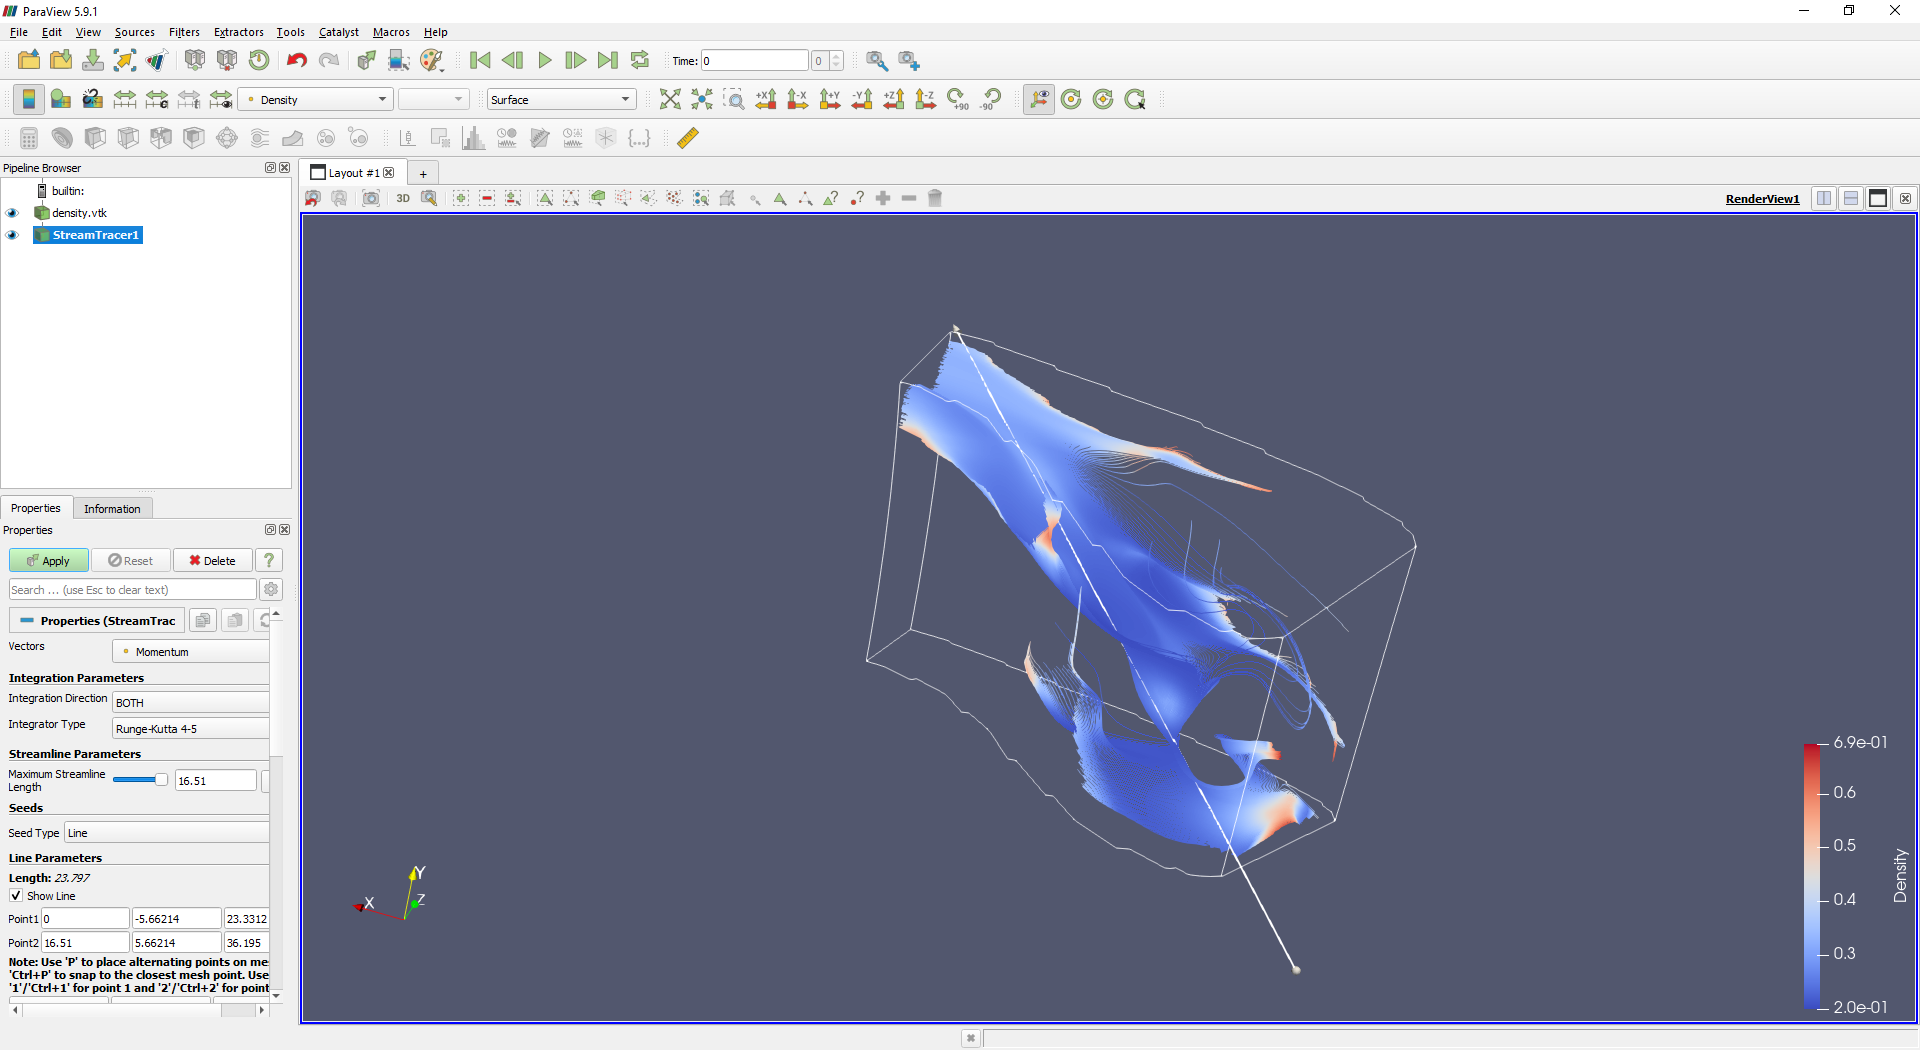
\includegraphics[width=\textwidth]{pictures/paraview.png}
    \caption{ParaView visualization of a StreamTracer using a structured grid point dataset.}
    \label{fig:paraview}
\end{figure}

Of the previous solutions, only Dreuning's work addresses the issue of allowing the creation of an integrated development environment in \acrshort{vr}. This is not an issue in and of itself, but it makes for a cumbersome and time consuming development environment for \acrshort{vr} applications. The solutions all miss one of the key characteristics we envision for our environment, be it the performances necessary for \acrshort{vr} applications, the generality of an \acrshort{ide} or the support for multiple \acrshort{hmd}s.
